\section{Experiment}
\label{sec:exper}


\subsection{Implementation Details}
We instantiate \ourmethod with a 7B-parameter Prismatic VLM backbone and a diffusion action expert with approximately 300M parameters.
\ourmethod receives a single third-person RGB observation resized to $224\times224$ together with the language instruction, and predicts continuous 7-DoF end-effector actions with an action chunk size of 16.
We train the model on 8 NVIDIA H800 GPUs using PyTorch FSDP.
Each GPU processes 32 samples, resulting in a global batch size of 256, and the learning rate is set to $2\times10^{-5}$.
Both the short-term and long-term memory vaults keep a maximum capacity of $L=16$ units.
The latent memory seeker retrieves the top $K\!=\!8$ units from each vault, and the latent memory condenser reconstructs the retrieved evidence into $L_\text{s}\!=\!8$ short-term memory tokens and $L_\text{l}\!=\!4$ long-term memory tokens.
The query builder $\mathcal{B}$ and the two memory formers $\mathcal{F}_\text{v}$ and $\mathcal{F}_\text{c}$ are implemented as two-layer transformer blocks with masked attention (more details in Appendix).
During inference, the diffusion action expert generates actions with DDIM~\cite{songdenoising} sampling using 10 denoising steps.

\begin{table}[t]
\centering
\caption{
\small\textbf{Quantitative comparison results on SimplerEnv-Bridge~\cite{li2025evaluating}} (\S\ref{sec:simpler}) with WidowX robot.}
\label{tab:simplerenv_bridge}
\resizebox{\linewidth}{!}{
\setlength\tabcolsep{10pt}
\renewcommand\arraystretch{1.0}
\begin{tabular}{l|c|cccc|c}
\thickhline
\rowcolor{mygray}
Method
& Publication
& \makecell{Spoon\\on Towel}
& \makecell{Carrot\\on Plate}
& \makecell{Stack\\Cube}
& \makecell{Eggplant\\in Basket}
& \makecell{Avg.\\Success} \\
\hline 
\hline
RT-1-X~\citep{o2024open}              & ICRA'24 & 0.0  & 4.2  & 0.0  & 0.0   & 1.1  \\
OpenVLA~\citep{kim2025openvla}             & CoRL'25 & 4.2  & 0.0  & 0.0  & 12.5  & 4.2  \\
TraceVLA~\citep{zheng2025tracevla}         & ICLR'25 & 12.5 & 16.6 & 16.6 & 65.0  & 27.7 \\
SpatialVLA~\citep{qu2025spatialvla}        & RSS'25  & 16.7 & 25.0 & 29.2 & 100.0 & 42.7 \\
Magma~\citep{yang2025magma}                & CVPR'25 & 37.5 & 29.2 & 20.8 & 91.7  & 44.8 \\
CogACT~\citep{li2024cogact}          & ArXiv'24 & 58.3 & 45.8 & 29.2 & 95.8  & 57.3 \\
$\pi_0$~\citep{black2024pi_0}          & CoRL'25& 83.8 & 52.5 & 52.5 & 87.9 & 69.2 \\
DreamVLA~\citep{zhang2026dreamvla}          & NeurIPS'25&45.8 &45.8 &25.0 &87.5 &51.0 \\
ThinkAct~\citep{huang2026thinkact}          & NeurIPS'25& 58.3& 37.5& 8.7 &70.8 &43.8 \\
CronusVLA~\citep{li2026towards}          & AAAI26& 66.7& 54.2& 20.8& 100.0& 60.4 \\
MemoryVLA~\citep{shi2025memoryvla}         & ICLR'26 & 75.0 & 75.0 & 37.5  & 100.0 & 71.9 \\
SemanticVLA~\citep{ni2026semanticvla}          & CVPR'26& 83.6 &54.5& 40.3& 81.8 &65.1\\
\hline 
\ourmethod~\textbf{(Ours)}
& --
& 83.3 & 75.0 & 41.7 & 95.8
& \textbf{73.9}\\
\hline
\end{tabular}
}
\end{table}

\subsection{Simulated  Evaluation on SimplerEnv-Bridge}
\label{sec:simpler}
\noindent\textbf{Training and Evaluation Protocol.}
SimplerEnv evaluates real-to-sim generalization of robot manipulation policies trained on real-world data.
We evaluate \ourmethod on the SimplerEnv-Bridge~\cite{li2025evaluating} suite under the standard Bridge protocol.
The policy is trained on the Bridge v2 dataset~\cite{walke2023bridgedata} for 50k optimization steps, with validation performed every 2.5k steps.
The final results are reported using the checkpoint that achieves the best validation performance. For evaluation, each task is tested over 24 trials, and we report the average success rate across trials.

\noindent\textbf{Evaluation Results.}
As shown in Table~\ref{tab:simplerenv_bridge}, \ourmethod achieves the highest average success rate of \textbf{73.9}\% on SimplerEnv-Bridge, yielding a \textbf{16.6} gain over the CogACT~\cite{li2024cogact} baseline and surpassing recent state-of-the-art VLAs such as $\pi_0$~\cite{black2024pi_0} and SemanticVLA~\citep{ni2026semanticvla}. Per task, \ourmethod obtains \textbf{83.3}\% \textit{on Put Spoon on Towel}, \textbf{75.0}\% on \textit{Put Carrot on Plate}, \textbf{41.7}\% on \textit{Stack Cube}, and \textbf{95.8}\% on \textit{Put Eggplant in Basket}. These results indicate that injecting dual latent memory tokens into the VLA reasoning sequence provides effective historical context for action prediction, improving manipulation performance and maintaining strong robustness across diverse task settings.

\subsection{Simulated  Evaluation on LIBERO}
\label{sec:libero}
\noindent\textbf{Training and Evaluation Protocol.}
We evaluate \ourmethod on the LIBERO~\cite{liu2023libero} benchmark using a Franka robot across five suites: spatial awareness (Spatial), object manipulation (Object), goal completion (Goal), and long-horizon reasoning (Long-10 and Long-90). The first four suites comprise 10 tasks each, while Long-90 contains 90 tasks. Following the OpenVLA protocol~\cite{kim2025openvla}, we use 50 demonstrations per task. We train separate models for Spatial, Object, and Goal for 20k optimization steps, and jointly train on Long-10 and Long-90 for 40k steps. During training, we evaluate checkpoints at 1k-step intervals and select the best-performing one according to validation success. We report success rates for each suite and the overall average over 50 rollouts per task.

\noindent\textbf{Evaluation Results.}
As shown in Table~\ref{tab:libero}, \ourmethod achieves the best overall performance on LIBERO, reaching an average success rate of \textbf{97.6}\% across the five suites.
It improves over the strongest reported memory-augmented method MemoryVLA~\citep{shi2025memoryvla}, by \textbf{1.1} points, and surpasses strong VLA baselines such as CogACT~\citep{li2024cogact} by \textbf{4.4} points.
Compared with $\pi_0$~\citep{black2024pi_0}, \ourmethod obtains a first-four-suite average of \textbf{97.7}\%, yielding a \textbf{3.5} point improvement.
Notably, these gains are achieved without the additional proprioceptive and wrist-camera inputs used by starred methods.
Across individual suites, \ourmethod consistently attains the highest success rates, with \textbf{98.8}\% on Spatial, \textbf{99.0}\% on Object, \textbf{97.2}\% on Goal, \textbf{95.8}\% on Long-10, and \textbf{97.0}\% on Long-90.
The improvements on the long-horizon suites are particularly important: \ourmethod outperforms MemoryVLA by \textbf{2.4} points on Long-10 and \textbf{1.4} points on Long-90.
These results suggest that weaving short-term visual evidence and long-term semantic memory directly into the VLA reasoning sequence helps the policy resolve temporally ambiguous states, preserve task progress, and generate more reliable actions for both general manipulation and long-horizon instruction following.

\begin{table}[t]
\centering
\caption{
\small\textbf{Quantitative comparison results on LIBERO~\citep{liu2023libero} (\S\ref{sec:libero}) with Franka robot.}
Success rates (\%) are reported across five suites.
$^{*}$ indicates methods using additional proprioceptive and wrist-camera inputs.
For methods without LIBERO-90 results, we report the average over the first four suites.
}
\vspace{-5pt}
\label{tab:libero}
\resizebox{\linewidth}{!}{
\setlength\tabcolsep{7pt}
\renewcommand\arraystretch{1.0}
\begin{tabular}{l|c|ccccc|c}
\thickhline
\rowcolor{mygray}
Method & Publication& Spatial & Object & Goal & Long-10 & Long-90 & \makecell{Avg. Success} \\
\hline
\hline
Diffusion Policy~\citep{chi2025diffusion} & RSS'23 & 78.3 & 92.5 & 68.3 & 50.5 & -- & 72.4 \\
Octo~\citep{octo_2023} & RSS'24 & 78.9 & 85.7 & 84.6 & 51.1 & -- & 75.1 \\
UniACT~\citep{zheng2025universal} & CVPR'25 & 77.0 & 87.0 & 77.0 & 70.0 & 73.0 & 76.8 \\
SpatialVLA~\citep{qu2025spatialvla} & RSS'25 & 88.2 & 89.9 & 78.6 & 55.5 & 46.2 & 71.7 \\
OpenVLA~\citep{kim2025openvla} & CoRL'25 & 84.7 & 88.4 & 79.2 & 53.7 & 73.5 & 75.9 \\
CoT-VLA~\citep{zhao2025cot} & CVPR'25 & 87.5 & 91.6 & 87.6 & 69.0 & -- & 83.9 \\
$\pi_0$-FAST$^{*}$~\citep{pertsch2025fast} & ArXiv'25 & 96.4 & 96.8 & 88.6 & 60.2 & 83.1 & 85.0 \\
CogACT~\citep{li2024cogact} & ArXiv'24 & 97.2 & 98.0 & 90.2 & 88.8 & 92.1 & 93.2 \\
$\pi_0^{*}$~\citep{black2024pi_0} & CoRL'25 & 96.8 & 98.8 & 95.8 & 85.2 & -- & 94.2 \\
ThinkAct~\citep{huang2026thinkact}    & NeurIPS'25&  88.3 &91.4& 87.1 &70.9 &-- &84.4 \\
MemoryVLA~\citep{shi2025memoryvla}         & ICLR'26 & 98.4& 98.4& 96.4 &93.4& 95.6& 96.5 \\
Fast-ThinkAct~\citep{huang2026fast}   & CVPR'26&92.0& 97.2& 90.2 &79.4& -- &89.7 \\
SemanticVLA~\citep{ni2026semanticvla}   & CVPR'26&98.0& 98.6& 96.8& 94.4& -- &97.0 \\
LARA~\citep{liu2026lara}   & ICML'26&96.5& 97.5& 96.0 &92.5& -- & 95.6\\
\hline
\ourmethod~\textbf{(Ours)} & -- & 98.8 & 99.0 & 97.2 & 95.8& 97.0& \textbf{97.6}\\
\hline
\end{tabular}
}
\vspace{-10pt}
\end{table}
\subsection{Ablation Study}
\label{sec:abation}
\noindent\textbf{Effectiveness of Dual-scale Latent Memory.}
We evaluate the contribution of each memory source by selectively removing it from the latent VLA input sequence.
We consider four settings: the full \ourmethod with both short-term and long-term latent memory, \textit{w/o Short-term Memory} that removes the visual-dominant memory tokens and only keeps long-term semantic memory, \textit{w/o Long-term Memory} that removes the long-term semantic memory tokens and only keeps short-term visual memory, and \textit{w/o Dual-scale Memory} that removes both memory streams. 
Table~\ref{tab:ablation_dual_memory} shows that the full dual-memory design achieves the best performance on both benchmarks, reaching \textbf{73.9}\% on SimplerEnv~\cite{li2025evaluating} and \textbf{97.0}\% on LIBERO-90~\cite{liu2023libero}.
Removing both memory streams causes the largest degradation, dropping performance to 57.3\% and 92.1\%, respectively.
These results suggest the complementary roles of the two vaults: short-term memory preserves current-episode visual evidence such as object states and transient perceptual cues, while long-term memory maintains task progress and action-continuity evidence over longer horizons.
Therefore, removing either stream should weaken temporally grounded action reasoning, and removing both streams should further reduce \ourmethod to a memory-free VLA policy.
\begin{table}[t]
\begin{minipage}[t]{0.49\linewidth}
\centering
\caption{
\small \textbf{Detailed analysis of dual-scale latent memory} on SimplerEnv~\cite{li2025evaluating} and LIBERO~\cite{liu2023libero} (\S\ref{sec:abation}).
}
\vspace{-5pt}
\label{tab:ablation_dual_memory}
\resizebox{\linewidth}{!}{
\setlength\tabcolsep{4pt}
\renewcommand\arraystretch{1.0}
\begin{tabular}{l|cc}
\thickhline
\rowcolor{mygray}
Method
& SimplerEnv
& LIBERO-90 \\
\hline
\hline
w/o Dual Memory       & 57.3 & 92.1 \\
w/o Short-term Memory  & 65.6 & 95.4  \\ 
w/o Long-term Memory & 64.6 & 94.8 \\\hline
\ourmethod~\textbf{(Ours)}
& \textbf{73.9} & \textbf{97.0} \\\hline

\end{tabular}
}



\end{minipage}
\hfill
\begin{minipage}[t]{0.5\linewidth}
\centering
\caption{\small \textbf{Ablation study of latent-native memory integration} on SimplerEnv~\cite{li2025evaluating} and LIBERO~\citep{liu2023libero} (\S\ref{sec:abation}).
}
\vspace{-5pt}
\label{tab:ablation_latent_native_memory}
\resizebox{\linewidth}{!}{
\setlength\tabcolsep{1.9pt}
\renewcommand\arraystretch{1.0}
\begin{tabular}{l|cc}
\thickhline
\rowcolor{mygray}
Method
& SimplerEnv
& LIBERO-90 \\
\hline
\hline
\textsc{Baseline}       & 57.3 & 92.1 \\
Policy-side Memory
& 71.9 & 94.8 \\
Raw Retrieval Conditioning
& 69.8 & 95.1 \\
\hline
\ourmethod~\textbf{(Ours)}
& \textbf{73.9} & \textbf{97.0} \\
\hline
\end{tabular}
}

\end{minipage}
\vspace{-5pt}
\end{table}
% \centering
\caption{
\small \textbf{Detailed analysis of dual-scale latent memory} on SimplerEnv~\cite{li2025evaluating} and LIBERO~\cite{liu2023libero} (\S\ref{sec:abation}).
}
\vspace{-5pt}
\label{tab:ablation_dual_memory}
\resizebox{\linewidth}{!}{
\setlength\tabcolsep{4pt}
\renewcommand\arraystretch{1.0}
\begin{tabular}{l|cc}
\thickhline
\rowcolor{mygray}
Method
& SimplerEnv
& LIBERO-90 \\
\hline
\hline
w/o Dual Memory       & 57.3 & 92.1 \\
w/o Short-term Memory  & 65.6 & 95.4  \\ 
w/o Long-term Memory & 64.6 & 94.8 \\\hline
\ourmethod~\textbf{(Ours)}
& \textbf{73.9} & \textbf{97.0} \\\hline

\end{tabular}
}



% \centering
\caption{\small \textbf{Ablation study of latent-native memory integration} on SimplerEnv~\cite{li2025evaluating} and LIBERO~\citep{liu2023libero} (\S\ref{sec:abation}).
}
\vspace{-5pt}
\label{tab:ablation_latent_native_memory}
\resizebox{\linewidth}{!}{
\setlength\tabcolsep{1.9pt}
\renewcommand\arraystretch{1.0}
\begin{tabular}{l|cc}
\thickhline
\rowcolor{mygray}
Method
& SimplerEnv
& LIBERO-90 \\
\hline
\hline
\textsc{Baseline}       & 57.3 & 92.1 \\
Policy-side Memory
& 71.9 & 94.8 \\
Raw Retrieval Conditioning
& 69.8 & 95.1 \\
\hline
\ourmethod~\textbf{(Ours)}
& \textbf{73.9} & \textbf{97.0} \\
\hline
\end{tabular}
}


\noindent\textbf{Latent-native Memory \textit{vs.} Policy-side Conditioning.}
We isolate the effect of memory consumption path in Table~\ref{tab:ablation_latent_native_memory}, where \textsc{Baseline} denotes the memory-free action policy without short-term and long-term memory.
The baseline reaches only 57.3\% on SimplerEnv~\cite{li2025evaluating} and 92.1\% on LIBERO-90~\cite{liu2023libero}, while adding memory as an external policy-side condition improves performance to 71.9\% and 94.8\%, respectively.
Directly feeding raw retrieved evidence to the action policy also improves over the baseline, but remains below the full model \ourmethod, suggesting that uncompressed retrieval can introduce redundant historical tokens.
By prepending compressed memory tokens as a memory-augmented VLA input sequence, \ourmethod enables action tokens to attend to latent memory, observation, and instruction in the same embedding space, achieving the best results of \textbf{73.9}\% and \textbf{97.0}\%.
These results confirm that the gain comes from latent-native memory integration rather than merely adding memory as external context.

\begin{wraptable}{r}{0.43\linewidth}
%\begin{table*}[t]
\vspace{-12pt}
\centering
\caption{
\small \textbf{Ablation study of the retrieved memory unit number $K$} on SimplerEnv~\cite{li2025evaluating} and LIBERO-90~\cite{liu2023libero} (\S\ref{sec:abation}).
}
\vspace{-8pt}
\label{tab:ablation_retrieved_k}
\resizebox{0.96\linewidth}{!}{
\setlength\tabcolsep{12pt}
\renewcommand\arraystretch{1.0}
\begin{tabular}{c|cc}
\thickhline
\rowcolor{mygray}
$K$
& SimplerEnv
& LIBERO-90 \\
\hline
\hline
$2$  & 66.7 & 94.4\\
$4$  & 70.8 & 95.9 \\
$8$  & \textbf{73.9} & \textbf{97.0} \\
$12$ & 71.8 & 96.2 \\
\hline
\end{tabular}
}
\vspace{-13pt}
\hspace{-2ex}
%\end{table*}
\end{wraptable}
\noindent\textbf{The Number of Retrieved Memory Units $K$.}
We further study how the retrieval budget of the memory seeker affects manipulation performance by varying the number of retrieved memory units per vault (Eq.~\ref{eq:short_memory_retrieval}).
Specifically, we evaluate $K \in \{2,4,8,12\}$ to examine how much historical evidence should be exposed to the condenser.
As shown in Table~\ref{tab:ablation_retrieved_k}, increasing the retrieval budget from $K\!=\!2$ to $K\!=\!4$ improves SR from 66.7\% to 70.8\% on SimplerEnv~\cite{li2025evaluating} and from 94.4\% to 95.9\% on LIBERO-90~\cite{liu2023libero}.
Further increasing the budget to $K\!=\!8$ yields the best performance, reaching \textbf{73.9}\% on SimplerEnv and \textbf{97.0}\% on LIBERO-90.
This indicates that a very small retrieval budget provides insufficient historical evidence for recovering task progress and transient visual changes.
However, using $K\!=\!12$ slightly reduces performance to 71.8\% and 96.2\%.
These results suggest that retrieving more memory units is beneficial to a moderate budget, while excessive retrieval can introduce redundant or weakly related evidence and increase the compression burden of the memory condenser.


\begin{wrapfigure}[13]{r}{0.64\textwidth}
\vspace{-.5cm}
        \hspace{+0.04cm}
        \centering
		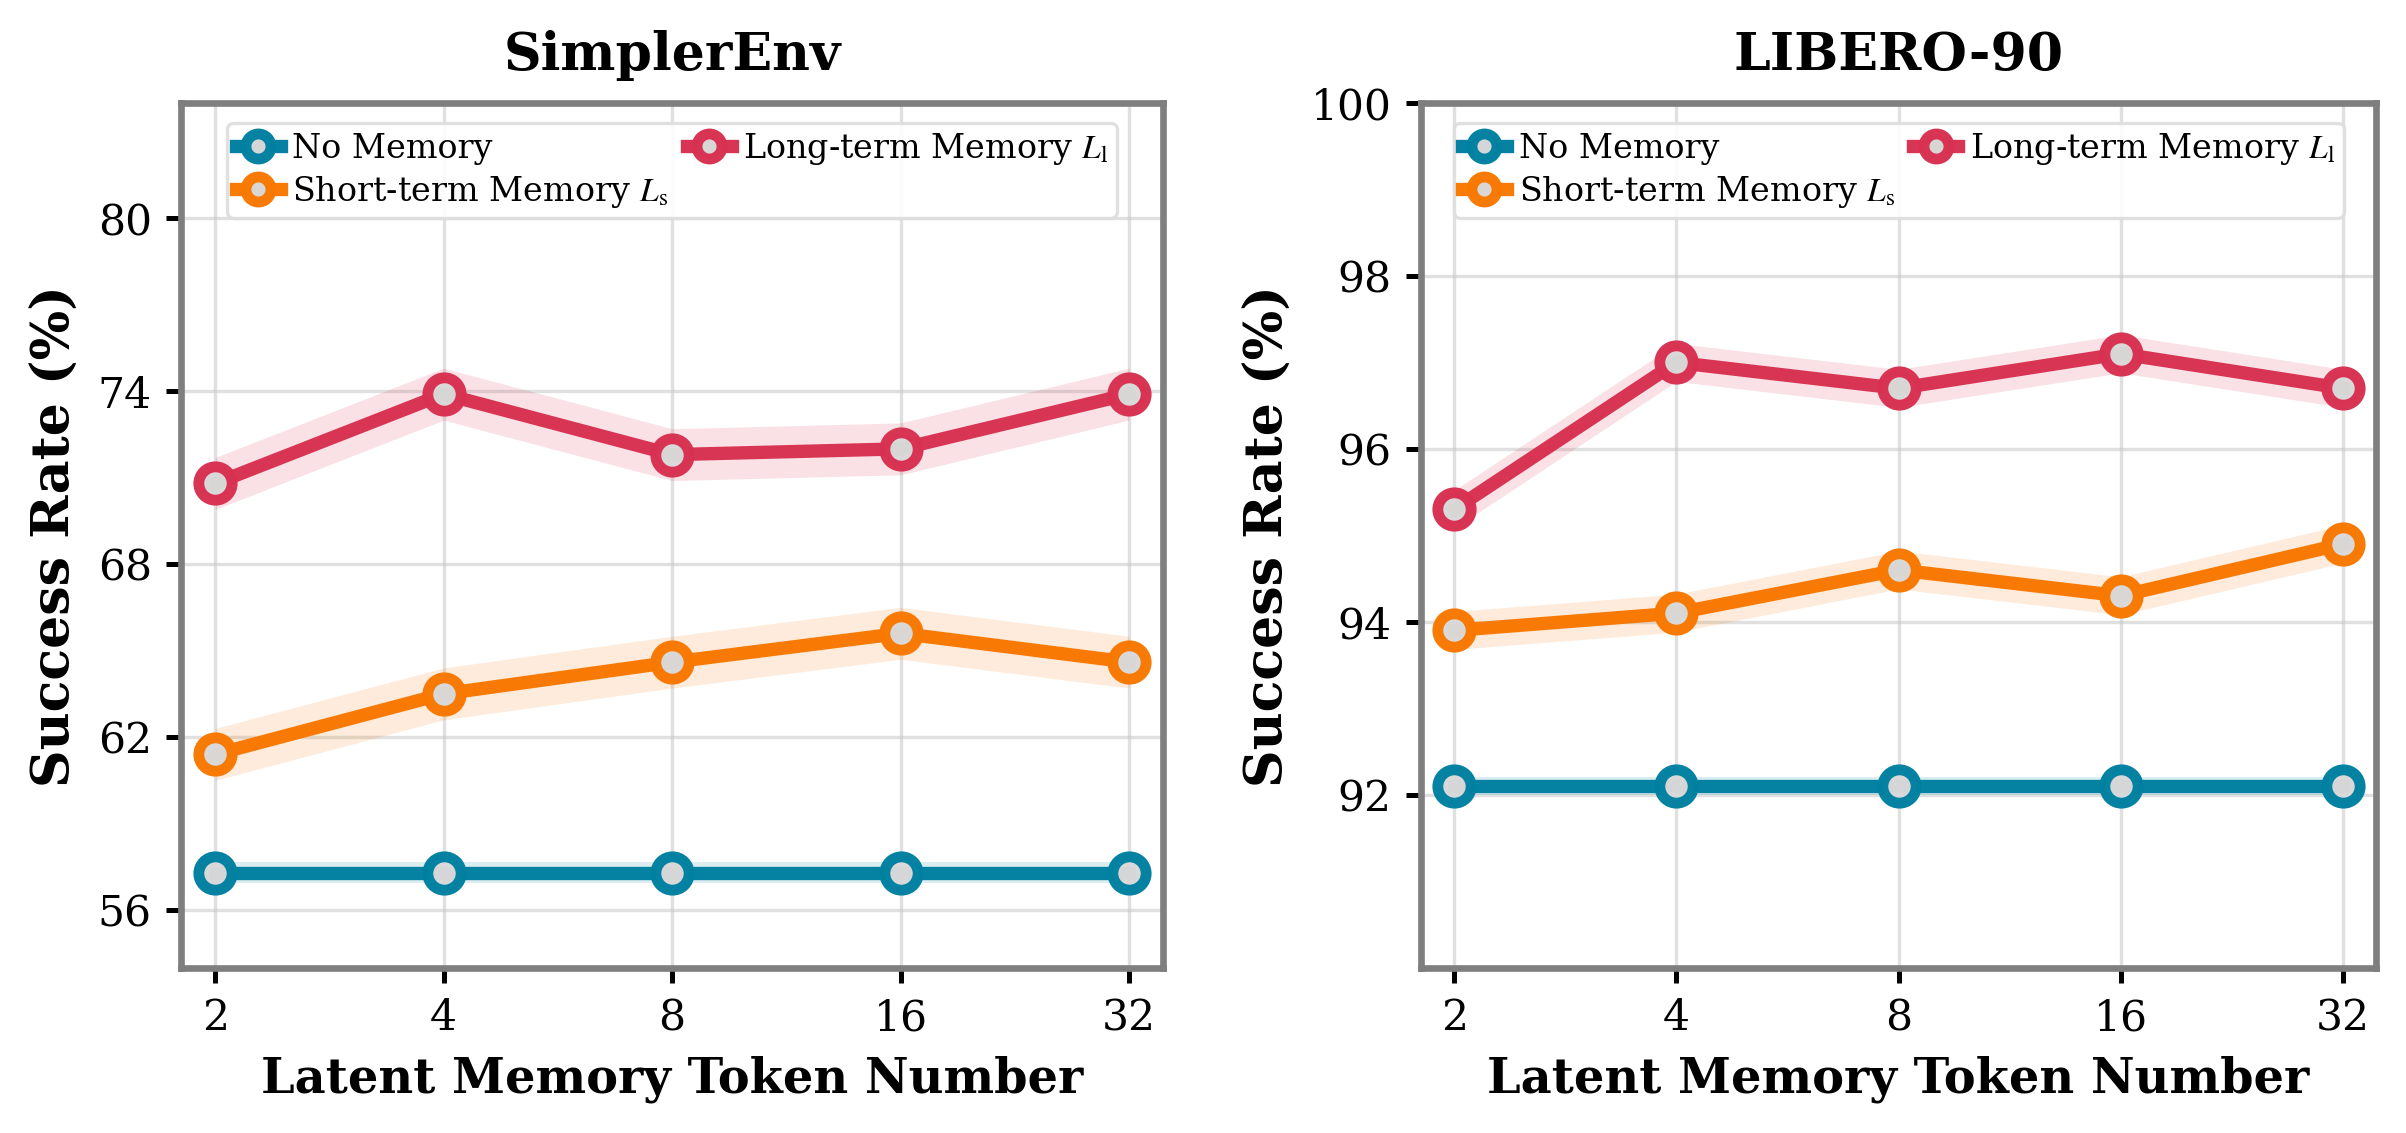
\includegraphics[width=1\linewidth]{figs/table6.png}
\captionsetup{font=small,width=1\linewidth}
 \vspace{-0.8cm}
	\caption{
\small \textbf{Ablation study of the latent memory token number} on SimplerEnv~\cite{li2025evaluating} and LIBERO-90~\cite{liu2023libero} (\S\ref{sec:abation}).
}
 \label{fig:latentnum}
\end{wrapfigure}
\noindent\textbf{The Number of Latent Memory Tokens $L_\text{s}$ and $L_\text{l}$.} 
We next investigate the impact of the short-term and long-term latent memory token number (Eq.~\ref{eq:memory_condensation}) in Fig.~\ref{fig:latentnum}.
For short-term memory, increasing $L_\text{s}$ from $2$ to $16$ raises SimplerEnv~\cite{li2025evaluating} SR from 61.4\% to 65.6\%, suggesting that more short-term latent memory tokens help preserve fine-grained perceptual evidence; the gain saturates when $L_\text{s}=32$.
For long-term memory, fixing $L_\text{s}=8$ and increasing long-term latent memory token number $L_\text{l}$ provides stronger task-progress and action-continuity cues, reaching up to 73.9\% on SimplerEnv~\cite{li2025evaluating} and 97.0\% on LIBERO-90~\cite{liu2023libero}.
Although larger latent memory token budgets can yield strong performance, they also lengthen the VLA self-attention context and increase computational costs; therefore, we use $(L_\text{s},L_\text{l})=(8,4)$ as a balanced default between performance and efficiency.


% \input{tabs/ablation_latent_memory_tokens.tex}

% External conditioning vs latent interweaving

% w/o seeker / latest-K / random retrieval / full seeker




% 记忆更新策略  效率比较




% \subsection{Real-world Evaluation}
% % \noindent\textbf{Data collection.}

% \noindent\textbf{Training and Evaluation Protocol.}
% We evaluate two real-robot suites, General and Long-horizon
% Temporal, on Franka and WidowX robots. Both use an Intel RealSense D435 RGB camera mounted
% in a fixed front view. Images are captured at 640 × 480 and downsampled to 224 × 224. The system
% is integrated via ROS. For General, each task uses 50-150 demonstrations and is evaluated from
% randomized initial states. Pick Diverse Fruits comprises five variants with 5 trials per variant (25
% total); all other General tasks use 15 trials. For Long-horizon Temporal, each task uses 200-300
% demonstrations and is evaluated with 10-15 trials using step-wise scoring to reflect progress over
% sub-goals. Training runs for approximately 5k–20k steps depending on the task and data size.  More details are provided in Appendix.

% \noindent\textbf{Evaluation Results.}
% As shown in Table 5, MemoryVLA achieves average success
% scores of 85\% on general tasks and 83\% on long-horizon temporal tasks, exceeding CogACT by
% +9 and +26 percentage points, respectively, and surpassing across both suites. On general tasks,
% it exceeds the strongest baseline on every task, with notable gains on Egg in Pan (+13) and Egg in
% Oven (+20). On long-horizon temporal tasks, improvements are larger, including +43 on Seq. Push
% Buttons, +38 on Change Food, +32 on Guess Where, and +17 on Clean Table  Count. These results
% demonstrate strong real-world competence and highlight the benefits of temporal memory.
